\subsection{Normalized No-load Angular Velocity Input}

We have the no-load dynamic model for the BLDC motor:
\begin{align*}
    J_m \dot \omega_m + (K_r K_v  + b_f) \omega_m + M_f &= u K_r V_{in}
\end{align*}
At steady state ($\dot \omega_m = 0$), the above equation becomes:
\begin{align*}
    (K_r K_v  + b_f) \omega_m + M_f &= u K_r V_{in}
\end{align*}
Substituting the non-linear input filter:
\begin{align*}
    (K_r K_v  + b_f) \omega_m + M_f &= g_u(u_p) K_r V_{in}\\
    \implies \frac{(K_r K_v  + b_f)}{K_r} \left(\frac{\omega_m}{V_{in}}\right) + \frac{M_f}{K_r V_{in}} &= g_u(u_p)
\end{align*}

\itbf{Definition}: Let, $u_{\omega}$ be the no-load angular velocity of the motor at unit supply voltage for the given pwm input ($u_p$). Also, let us call it "\itbf{Normalized no-load angular velocity}".
\begin{align*}
    u_{\omega} &= \frac{\omega_m}{V_{in}} \text{  at  } u_p
\end{align*}
Thus,
\begin{align*}
    \left(\frac{K_r K_v  + b_f}{K_r} \right) u_{\omega} &+ \frac{M_f}{K_r V_{in}} = g_u(u_p)\\
    \implies u_{\omega} &= \left(\frac{K_r}{K_r K_v  + b_f} \right) \left( g_u(u_p) - \frac{M_f}{K_r V_{in}} \right)\\
    &= \left(\frac{K_r}{K_r K_v  + b_f} \right) g_u(u_p) - \left(\frac{1}{K_r K_v  + b_f} \right) \frac{M_f}{V_{in}}
\end{align*}
Assuming, the supply voltage will not be varying much and the variation will be captured in the input uncertainity. Let $V_{in}$ on the RHS be $\hat V_{in}$. thus:
\begin{align*}
    u_{\omega} &= \left(\frac{K_r}{K_r K_v  + b_f} \right) g_u(u_p) - \left(\frac{1}{K_r K_v  + b_f} \right) \frac{M_f}{\hat V_{in}}
\end{align*}
Let,
\begin{align*}
    g_w (u_p) &= \left(\frac{K_r}{K_r K_v  + b_f} \right) g_u(u_p) - \left(\frac{1}{K_r K_v  + b_f} \right) \frac{M_f}{\hat V_{in}}
\end{align*}
The parmeters of assumed structure of $g_w(.)$ are estimatable form the experimental data ($\omega, u_p$) unlike $g_u$. Though, this method introduces additional uncertainity because of the $\hat V_{in}$, but it can be justifiably assumed to be far less than the uncertainity due to fitting ($\omega-u_p$) curve with for $g_w(.)$.

Writing, $u_{\omega}$ interms of actual PWM input to the motor $u$.
\begin{align*}
    u_{\omega} &= \left(\frac{K_r}{K_r K_v  + b_f} \right) u - \left(\frac{1}{K_r K_v  + b_f} \right) \frac{M_f}{\hat V_{in}}
\end{align*}
\begin{equation}
    \implies K_r u = (K_r K_v  + b_f) u_\omega + \frac{M_f}{\hat V_{in}}
    \label{eqn:norm_in}
\end{equation}
Thus, $u_{\omega}$ is $u$ scaled lineraly.

\subsubsection{Logarithmic form for $g_w(.)$ and Parameter Estimation}

Based on the experimental data, $g_w(.)$ is assumed to have the following logarithmic (natural-log) form:
\begin{align*}
    g_w(u_p) &= a \ln(u_p - 1110) + b
\end{align*}
The choice of bias as $1110$ was due to the fact that the maximum input that can be given to the esc-motor sytem with no response is 1110. The values of $a, b$ are obtained by lineraly fitting $u_\omega$ to $u_p$.

\begin{figure}[H]
    \centering
    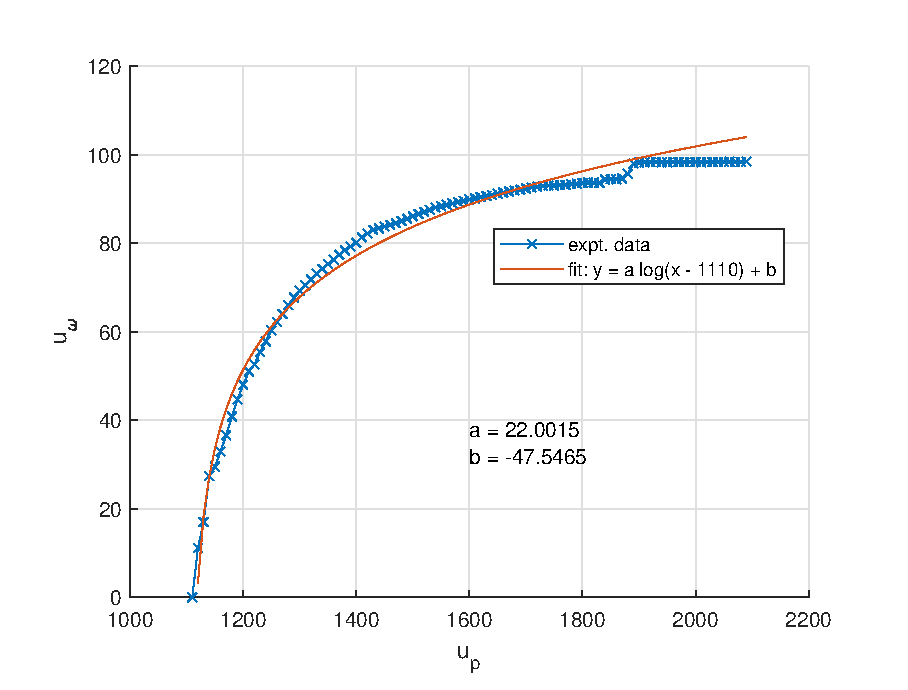
\includegraphics[width = 0.7\textwidth]{./figs/norm_omega/g_w.eps}
    \caption{Logarithmic fit for $g_w()$}
\end{figure}
Thus,
\begin{align*}
    \boxed{g_w(u_p) = 22 \ln(u_p - 1110)- 47.5 }
\end{align*}
and,
\begin{align*}
    g'_w(u_p) = \frac{22}{u_p - 1110}
\end{align*}


\subsubsection{Static mapping with propeller}
Form eqn.~\ref{eqn:prop} and introducing the normalized input from eqn.~\ref{eqn:norm_in}:
\begin{align*}
    J\dot \omega + (K_rK_v + b_f) \omega + C_D \omega^2 + M_f = u K_r V_{in}
\end{align*}
